
%(BEGIN_QUESTION)
% Copyright 2012, Tony R. Kuphaldt, released under the Creative Commons Attribution License (v 1.0)
% This means you may do almost anything with this work of mine, so long as you give me proper credit

Suppose you are asked to build a complete control system using a DP transmitter, Honeywell UDC2000 PID controller, an air-to-open control valve (with positioner), and an I/P transducer:

$$\includegraphics[width=15.5cm]{i00432x01.eps}$$

Sketch the necessary tube and wire connections to make this a working system.  Feel free to add any other components as needed.

\vfil 

\underbar{file i00432}
\eject
%(END_QUESTION)





%(BEGIN_ANSWER)

This is a graded question -- no answers or hints given!
 
%(END_ANSWER)





%(BEGIN_NOTES)

The addition of a 24 VDC power supply and 250 $\Omega$ resistor are both necessary to make this a working control loop:

$$\includegraphics[width=15.5cm]{i00432x02.eps}$$

We know that an external power supply is necessary (rather than being built into the controller itself) because of how the controller's PV input is labeled ``1-5 volt''.  This tells us the controller input is basically functioning as a voltage-sensing instrument (i.e. a voltmeter).  As such, there is no way loop power could also be present at these same two terminals without negating their role as voltage-sensing inputs.  The only time one will ever see a built-in DC loop power supply in an indicating or controlling instrument is if that instrument's PV input signal is {\it current}, not voltage!

\vskip 10pt

A 250 ohm resistor is necessary to convert the transmitter's 4-20 mA current into a 1-5 VDC signal the controller can read.  Likewise, the controller's input terminals 8 and 7 must be connected in {\it parallel} with this resistor to measure its voltage (because voltage guaranteed to be the same among parallel-connected components) and the resistor must be connected in {\it series} with the transmitter (because current is guaranteed to be the same among series-connected components).

Important principles to keep in mind are electrical {\it sources} versus electrical {\it loads}.  The controller's current output is a source.  Loads include the I/P, the 250 ohm resistor, and the controller input itself (albeit a very light load, as it draws practically no current in its voltage-sensing function).  The necessity of a 24 volt loop power supply on the input wiring is evident by the fact that none of the other components comprising that circuit are sources, so there needs to be a source to motivate the 4-20 mA current to flow.  This is also the same reason the output circuit requires no 24 VDC source: the controller current output already functions as a source, and therefore the I/P may be wired directly to the controller output terminals.

%INDEX% Pictorial circuit review (analog signal wiring to process controller and positioner tubing)

%(END_NOTES)


